%% abtex2-modelo-artigo.tex, v-1.9.7 laurocesar
%% Copyright 2012-2018 by abnTeX2 group at http://www.abntex.net.br/ 
%%
%% This work may be distributed and/or modified under the
%% conditions of the LaTeX Project Public License, either version 1.3
%% of this license or (at your option) any later version.
%% The latest version of this license is in
%%   http://www.latex-project.org/lppl.txt
%% and version 1.3 or later is part of all distributions of LaTeX
%% version 2005/12/01 or later.
%%
%% This work has the LPPL maintenance status `maintained'.
%% 
%% The Current Maintainer of this work is the abnTeX2 team, led
%% by Lauro César Araujo. Further information are available on 
%% http://www.abntex.net.br/
%%
%% This work consists of the files abntex2-modelo-artigo.tex and
%% abntex2-modelo-references.bib
%%

% ------------------------------------------------------------------------
% ------------------------------------------------------------------------
% abnTeX2: Modelo de Artigo Acadêmico em conformidade com
% ABNT NBR 6022:2018: Informação e documentação - Artigo em publicação 
% periódica científica - Apresentação
% ------------------------------------------------------------------------
% ------------------------------------------------------------------------

\documentclass[
% -- opções da classe memoir --
article,			% indica que é um artigo acadêmico
11pt,				% tamanho da fonte
oneside,			% para impressão apenas no recto. Oposto a twoside
a4paper,			% tamanho do papel. 
% -- opções da classe abntex2 --
%chapter=TITLE,		% títulos de capítulos convertidos em letras maiúsculas
%section=TITLE,		% títulos de seções convertidos em letras maiúsculas
%subsection=TITLE,	% títulos de subseções convertidos em letras maiúsculas
%subsubsection=TITLE % títulos de subsubseções convertidos em letras maiúsculas
% -- opções do pacote babel --
english,			% idioma adicional para hifenização
brazil,				% o último idioma é o principal do documento
sumario=tradicional
]{abntex2}


% ---
% PACOTES
% ---

% ---
% Pacotes fundamentais 
% ---
\usepackage{lmodern}			% Usa a fonte Latin Modern
\usepackage[T1]{fontenc}		% Selecao de codigos de fonte.
\usepackage[utf8]{inputenc}		% Codificacao do documento (conversão automática dos acentos)
\usepackage{indentfirst}		% Indenta o primeiro parágrafo de cada seção.
\usepackage{nomencl} 			% Lista de simbolos
\usepackage{color}				% Controle das cores
\usepackage{graphicx}			% Inclusão de gráficos
\usepackage{microtype} 			% para melhorias de justificação
% ---

% ---
% Pacotes adicionais, usados apenas no âmbito do Modelo Canônico do abnteX2
% ---
\usepackage{lipsum}				% para geração de dummy text
% ---

% ---
% Pacotes de citações
% ---
\usepackage[brazilian,hyperpageref]{backref}	 % Paginas com as citações na bibl
\usepackage[alf]{abntex2cite}	% Citações padrão ABNT
% ---

% ---
% Configurações do pacote backref
% Usado sem a opção hyperpageref de backref
\renewcommand{\backrefpagesname}{Citado na(s) página(s):~}
% Texto padrão antes do número das páginas
\renewcommand{\backref}{}
% Define os textos da citação
\renewcommand*{\backrefalt}[4]{
	\ifcase #1 %
	Nenhuma citação no texto.%
	\or
	Citado na página #2.%
	\else
	Citado #1 vezes nas páginas #2.%
	\fi}%
% ---

% --- Informações de dados para CAPA e FOLHA DE ROSTO ---
\titulo{Tutorial de Desenvolvimento com FrameWeb SPA}
\tituloestrangeiro{FrameWeb SPA Development Tutorial}

\autor{
	Pedro Henrique Brunoro Hoppe\thanks{``Mestrando.'' \url{pedrohoppe@gmail.com}} 
	\\[0.5cm] 
	Vitór Estêvao Silva Souza\thanks{``Constar currículo sucinto de cada autor, com 
		vinculação corporativa e endereço de contato.''} }

\local{Brasil}
\data{2022}
% ---

% ---
% Configurações de aparência do PDF final

% alterando o aspecto da cor azul
\definecolor{blue}{RGB}{41,5,195}

% informações do PDF
\makeatletter
\hypersetup{
	%pagebackref=true,
	pdftitle={\@title}, 
	pdfauthor={\@author},
	pdfsubject={Modelo de artigo científico com abnTeX2},
	pdfcreator={LaTeX with abnTeX2},
	pdfkeywords={abnt}{latex}{abntex}{abntex2}{atigo científico}, 
	colorlinks=true,       		% false: boxed links; true: colored links
	linkcolor=blue,          	% color of internal links
	citecolor=blue,        		% color of links to bibliography
	filecolor=magenta,      		% color of file links
	urlcolor=blue,
	bookmarksdepth=4
}
\makeatother
% --- 

% ---
% compila o indice
% ---
\makeindex
% ---

% ---
% Altera as margens padrões
% ---
\setlrmarginsandblock{3cm}{3cm}{*}
\setulmarginsandblock{3cm}{3cm}{*}
\checkandfixthelayout
% ---

% --- 
% Espaçamentos entre linhas e parágrafos 
% --- 

% O tamanho do parágrafo é dado por:
\setlength{\parindent}{1.3cm}

% Controle do espaçamento entre um parágrafo e outro:
\setlength{\parskip}{0.2cm}  % tente também \onelineskip

% Espaçamento simples
\SingleSpacing


% ----
% Início do documento
% ----
\begin{document}
	
	% Seleciona o idioma do documento (conforme pacotes do babel)
	%\selectlanguage{english}
	\selectlanguage{brazil}
	
	% Retira espaço extra obsoleto entre as frases.
	\frenchspacing 
	
	% ----------------------------------------------------------
	% ELEMENTOS PRÉ-TEXTUAIS
	% ----------------------------------------------------------
	
	%---
	%
	% Se desejar escrever o artigo em duas colunas, descomente a linha abaixo
	% e a linha com o texto ``FIM DE ARTIGO EM DUAS COLUNAS''.
	% \twocolumn[    		% INICIO DE ARTIGO EM DUAS COLUNAS
	%
	%---
	
	% página de titulo principal (obrigatório)
	\maketitle
	
	
	% titulo em outro idioma (opcional)
	
	% ----------------------------------------------------------
	% ELEMENTOS TEXTUAIS
	% ----------------------------------------------------------
	\textual
	
	% ----------------------------------------------------------
	% Introdução
	% ----------------------------------------------------------
\section{Instalação}
	
\subsection{Instalação do FrameWeb SPA}
Para instalar o FrameWeb SPA acesse o sítio eletrônico \url{https://github.com/pedrohbh/FrameWebSPA} e clone o repositório para sua máquina (ou baixe o zip disponível em ``Code'' -> ``Download Zip'') [\autoref{fig:tutorial-1}].

\begin{figure}
	\centering
	\includegraphics[width=\linewidth]{"figuras/Tutorial 1"}
	\caption{Repositório GitHub}
	\label{fig:tutorial-1}
\end{figure}

Após baixar o repositório, siga os seguintes passos:
\begin{enumerate}
	\item Abra o Eclipse;
	\item Clique no menu Help -> Install New Software...;
	\item Clique em ``Add...'' (\autoref{fig:siriustuto516});
	\item Preencha os campos:
	\begin{description}
		\item[Name:] Pode ser o nome que você quiser. \textit{Sugestão: FrameWeb SPA};
		\item[Location:] Clique no botão ``Archive…'' e depois selecione o arquivo ``FrameWeb.zip'' na pasta onde foi clonado o repositório do GitHub anteriormente;
	\end{description}
	\item Clique no botão ``Add'' (\autoref{fig:tutorial-2});
	\item Em ``Work with:'' selecione o repositório adicionado no passo anterior (no nosso caso, \textit{FrameWeb SPA}), marque as opções ``FrameWeb Code Generator'' e ``FrameWeb Graphical Editor'' e clique em ``Next >'' (\autoref{fig:tutorial-3});
	\item Caso não apareçam as opções como na \autoref{fig:tutorial-3}, desmarque a opção ``Group items by category'';
	\item Siga os demais passos de instalação aceitando os termos de licença (\autoref{fig:licenca}). Caso apareça uma mensagem dizendo que os certificados de segurança não são reconhecidos, apenas marque todos e clique em Ok (\autoref{fig:certificado});
	\item Após a instalação, reinicie o Eclipse.
\end{enumerate}

\begin{figure}
	\centering
	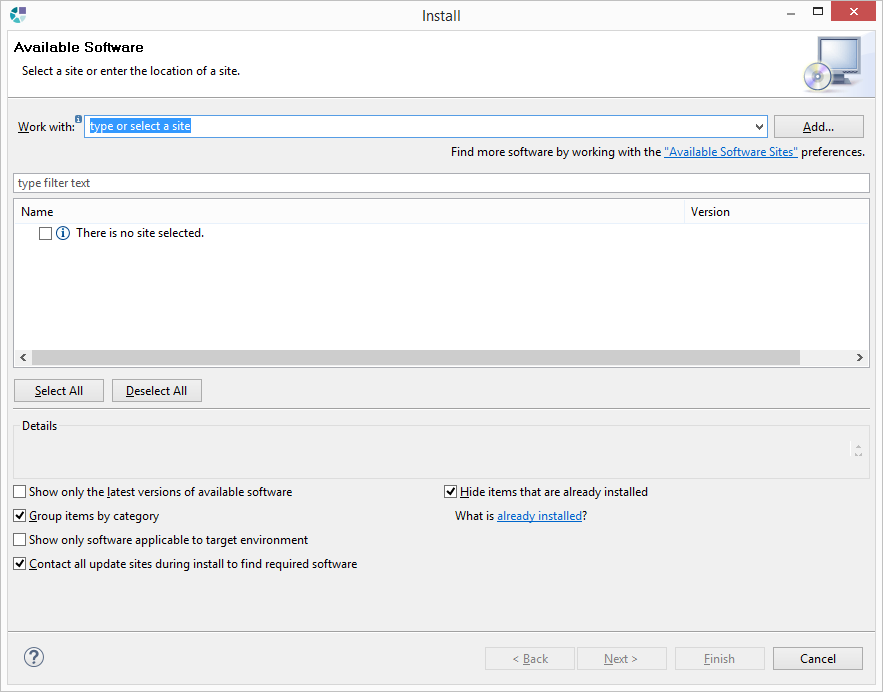
\includegraphics[width=0.7\linewidth]{figuras/Sirius_tuto5_16}
	\caption{Menu de instalação do Eclipse}
	\label{fig:siriustuto516}
\end{figure}

\begin{figure}
	\centering
	\includegraphics[width=0.7\linewidth]{"figuras/Tutorial 2"}
	\caption{Passo 5}
	\label{fig:tutorial-2}
\end{figure}

\begin{figure}
	\centering
	\includegraphics[width=0.7\linewidth]{"figuras/Tutorial 3"}
	\caption{Passo 6}
	\label{fig:tutorial-3}
\end{figure}

\begin{figure}
	\centering
	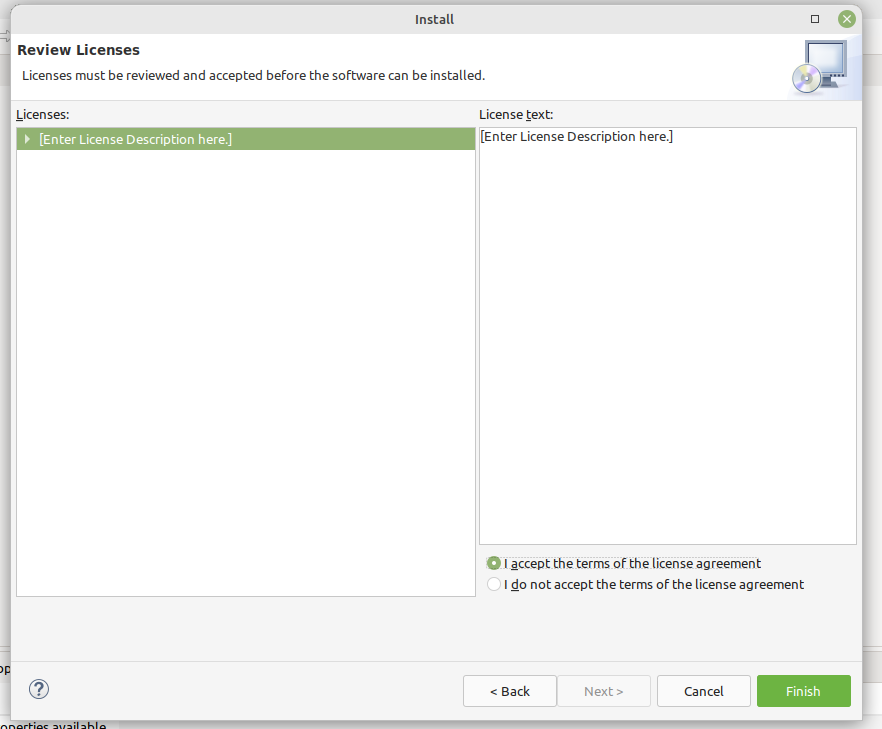
\includegraphics[width=0.7\linewidth]{figuras/licenca}
	\caption{Licença}
	\label{fig:licenca}
\end{figure}

\begin{figure}
	\centering
	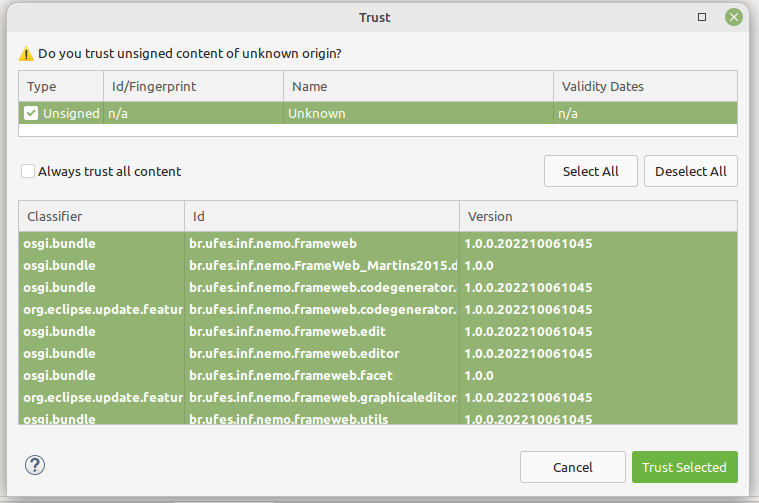
\includegraphics[width=0.7\linewidth]{figuras/certificado}
	\caption{Certificado}
	\label{fig:certificado}
\end{figure}


Após a instalação, a montagem do seu projeto segue os mesmos passos disponíveis na Wiki do FrameWeb \url{https://github.com/nemo-ufes/FrameWeb/wiki/ToolsTutorial02}. A \textbf{exceção} é a inclusão do projeto de arquitetura do seu framework, que ao invés de você baixar o JButler da página Github, você usará um dos três frameworks, a saber, Angular, React ou VueJS que estão disponíveis na pasta ``Frameworks'' no repositório clonado anteriormente \url{https://github.com/pedrohbh/FrameWebSPA}. Importe também a definição da linguagem Java dentro da pasta ``Language''.


%Open Eclipse;
%Click on the menu Help > Install New Software...
%In the Work with: field, type http://dev.nemo.inf.ufes.br/framewebplugin/ and press Enter;
%Unmark the checkbox Group items by category;
%Mark the checkbox for all FrameWeb Tools that show in the list (see figure below);
%Click Next twice, select the I accept the terms of the license agreement option and then click Finish;
%After the installation, restart Eclipse.



\section{Desenvolvimento}
O desenvolvimento do projeto seguem as mesmas instruções da Wiki \url{https://github.com/nemo-ufes/FrameWeb/wiki} para todos os modelos. A exceção é o Modelo de Navegação que também segue as mesmas instruções, porém com algumas mudanças que serão descritas a seguir.
	
\subsection{Partial}

O elemento novo principal é o Partial (\autoref{fig:partial}). Ele representa a parte gráfica de um \textit{component} SPA. Possui as mesmas características do elemento <<page>> para os Frameworks MVC tradicionais, porém sua interpretação (inclusive para o gerador de código) difere de <<Page>> e para o caso dos frameworks SPA, o Partial deve ser utilizado ao invés de Page.

\begin{figure}
	\centering
	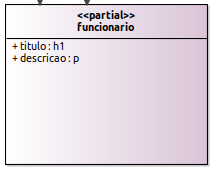
\includegraphics[width=0.4\linewidth]{figuras/Partial}
	\caption{O elemento Partial}
	\label{fig:partial}
\end{figure}


Como ``Components'' para os frameworks SPA obrigatoriamente tem uma parte gráfica e uma parte lógica (o controlador frontal), e por isso \textbf{todo partial tem que estar ligado a controlador frontal por meio da relação ``Front Controller Depedency''} como na \autoref{fig:partial4}, mesmo que não haja nenhum método específico que o controle. Observe também que os nomes dos pacotes (tanto do ``View Package'' onde está o partial como o ``Controller Package'' onde está o ``FrontControllerClass'') são iguais. Isso porque o ``Component'' está em um arquivo só, contendo o ``Partial'' e a parte de controlador frontal representado pelo ``FrontControllerClass''. Por isso é recomendado que se use o mesmo nome para cada ``Component'' (tanto de pacotes como para o nome do ``Partial'' e do ``FrontControllerClass'').

\begin{figure}
	\centering
	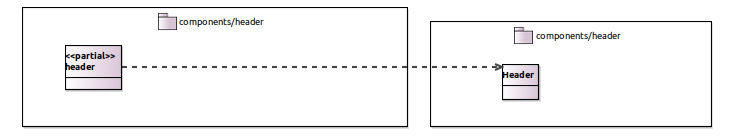
\includegraphics[width=0.7\linewidth]{figuras/Partial4}
	\caption{Partial ligado a seu FrontControllerClass}
	\label{fig:partial4}
\end{figure}

Os ``Partials'', assim como os ``Pages'', podem ter associado-lhes um formulário (``Form'', que no caso do FrameWeb é chamado de ``UIComponent'') e funcionam da mesma forma que em ``Pages'' (\autoref{fig:partial2}).

No caso de frameworks SPA, é comum que um método do controlador frontal retorne a si mesmo (a sua própria ``página''), por isso, ao contrário dos frameworks MVC tradicionais, não é obrigatório especificar um retorno do controlador frontal por meio do ``ResultDepedency'', apenas caso haja um redirecionamento para um outro ``Partial'' que não seja ele próprio.

\begin{figure}
	\centering
	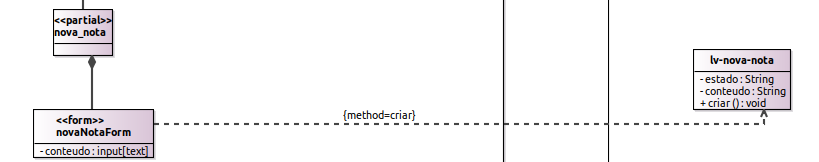
\includegraphics[width=0.7\linewidth]{figuras/Partial2}
	\caption{Partial ligado a um formulário}
	\label{fig:partial2}
\end{figure}

Falando em ``ResultDependecy'', ele que é o responsável por indicar o redirecionamento entre ``partials'' (observe a \autoref{fig:partial5}, o ``Partial'' menu possui um redirecionamento para o ``Partial'' departamento).

\begin{figure}
	\centering
	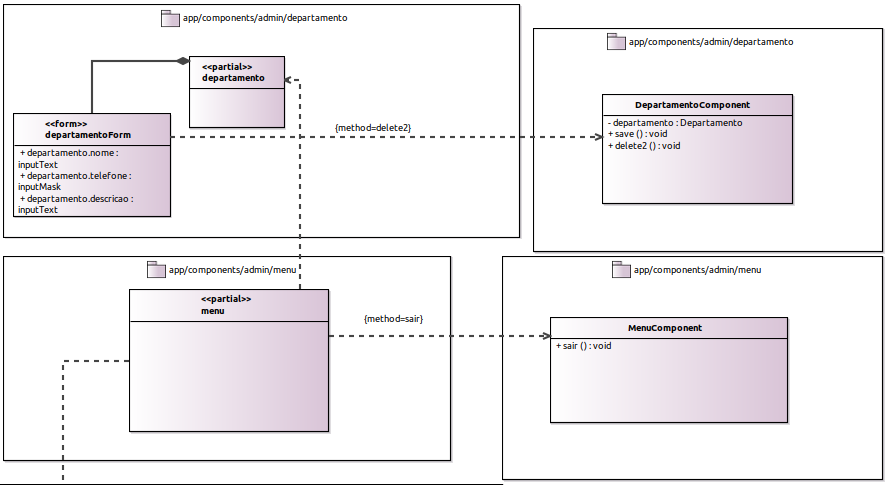
\includegraphics[width=0.7\linewidth]{figuras/Partial5}
	\caption{Exemplo de parte do sistema com redirecionamento}
	\label{fig:partial5}
\end{figure}


\subsection{Navigation Aggregation Association}	

Then we move on to the Navigation Model, creating a View Package /core/registration/ and a Controller Package br.ufes.informatica.oldenburg.core.controller. Here are some tips to create a Navigation Model:

Create pages using the Page component at the palette and give them a name without the .xhtml extension, as this will be added later by the code generator;

Create forms using the UI Component component at the palette. Form fields are created with UIComponentField and their type should be one of the tags from your visual component library (in our case, PrimeFaces);

When selecting the type of the tag from the dropdown list, if you type the name of the Tag the list will be filtered, but you have to start from the beginning (e.g., type Tag input to see the different PrimeFaces tags that start with input);

Form fields (UIComponentField) can also be added to pages directly;
To link a page to a form, use the Navigation Association component from the palette (I know, these names are not intuitive at all, we'll work on that...);

Moving to the controller side, a Front Controller Class can get attributes via IOParameter component and methods via Front Controller Method component from the palette;

To connect a page or form to a controller, use Front Controller Dependency and select one of the methods from the controller in the the Method property;

To connect a controller to a page, use the Result Dependency and select one of the methods from the controller in the the Result Method property. Further, click on the Result Constraints section and set the result and AJAX constraints if applicable.

Naming convention note: JButler templates expect all controller classes to have the Controller suffix (e.g., RegistrationController). Code generation will work better if you follow this naming convention.

The figure below shows the result for the Navigation Model.

	\section{Considerações finais}
	
	\lipsum[1]
	
	\begin{citacao}
		\lipsum[2]
	\end{citacao}
	
	\lipsum[3]
	
	% ----------------------------------------------------------
	% ELEMENTOS PÓS-TEXTUAIS
	% ----------------------------------------------------------
	\postextual
	
	% ----------------------------------------------------------
	% Referências bibliográficas
	% ----------------------------------------------------------
	\bibliography{abntex2-modelo-references}
	
	% ----------------------------------------------------------
	% Glossário
	% ----------------------------------------------------------
	%
	% Há diversas soluções prontas para glossário em LaTeX. 
	% Consulte o manual do abnTeX2 para obter sugestões.
	%
	%\glossary
	
	% ----------------------------------------------------------
	% Apêndices
	% ----------------------------------------------------------
	
	% ---
	% Inicia os apêndices
	% ---
	\begin{apendicesenv}
		
		% ----------------------------------------------------------
		\chapter{Nullam elementum urna vel imperdiet sodales elit ipsum pharetra ligula
			ac pretium ante justo a nulla curabitur tristique arcu eu metus}
		% ----------------------------------------------------------
		\lipsum[55-56]
		
	\end{apendicesenv}
	% ---
	
	% ----------------------------------------------------------
	% Anexos
	% ----------------------------------------------------------
	\cftinserthook{toc}{AAA}
	% ---
	% Inicia os anexos
	% ---
	%\anexos
	\begin{anexosenv}
		
		% ---
		\chapter{Cras non urna sed feugiat cum sociis natoque penatibus et magnis dis
			parturient montes nascetur ridiculus mus}
		% ---
		
		\lipsum[31]
		
	\end{anexosenv}
	
	% ----------------------------------------------------------
	% Agradecimentos
	% ----------------------------------------------------------
	
	\section*{Agradecimentos}
	Texto sucinto aprovado pelo periódico em que será publicado. Último 
	elemento pós-textual.
	
\end{document}
